
\chapter{関連システム}
\label{chap:relatedSystem}

本章では、関連するシステムについて解説し、簡素化支援システムとの類似性や参考点などについて述べる。

\newpage

\section{映像作品『Augmented City 3D』における日常でのAR利用}

Keiichi Mastuda氏のデザインフィクションコンセプト映画の『Augumented City 3D』(2010)\cite{arcity}では、カフェテリアで自身のPC環境を開くような描写がある(図\ref{fig:arcity01})。PCディスプレイ及びキーボードやマウスなどが仮想的に代替され、どのような環境であっても再現することができるという点で、簡素化支援システムとの類似性がある。

\begin{figure}[htbp]
  \begin{center}
     \fbox{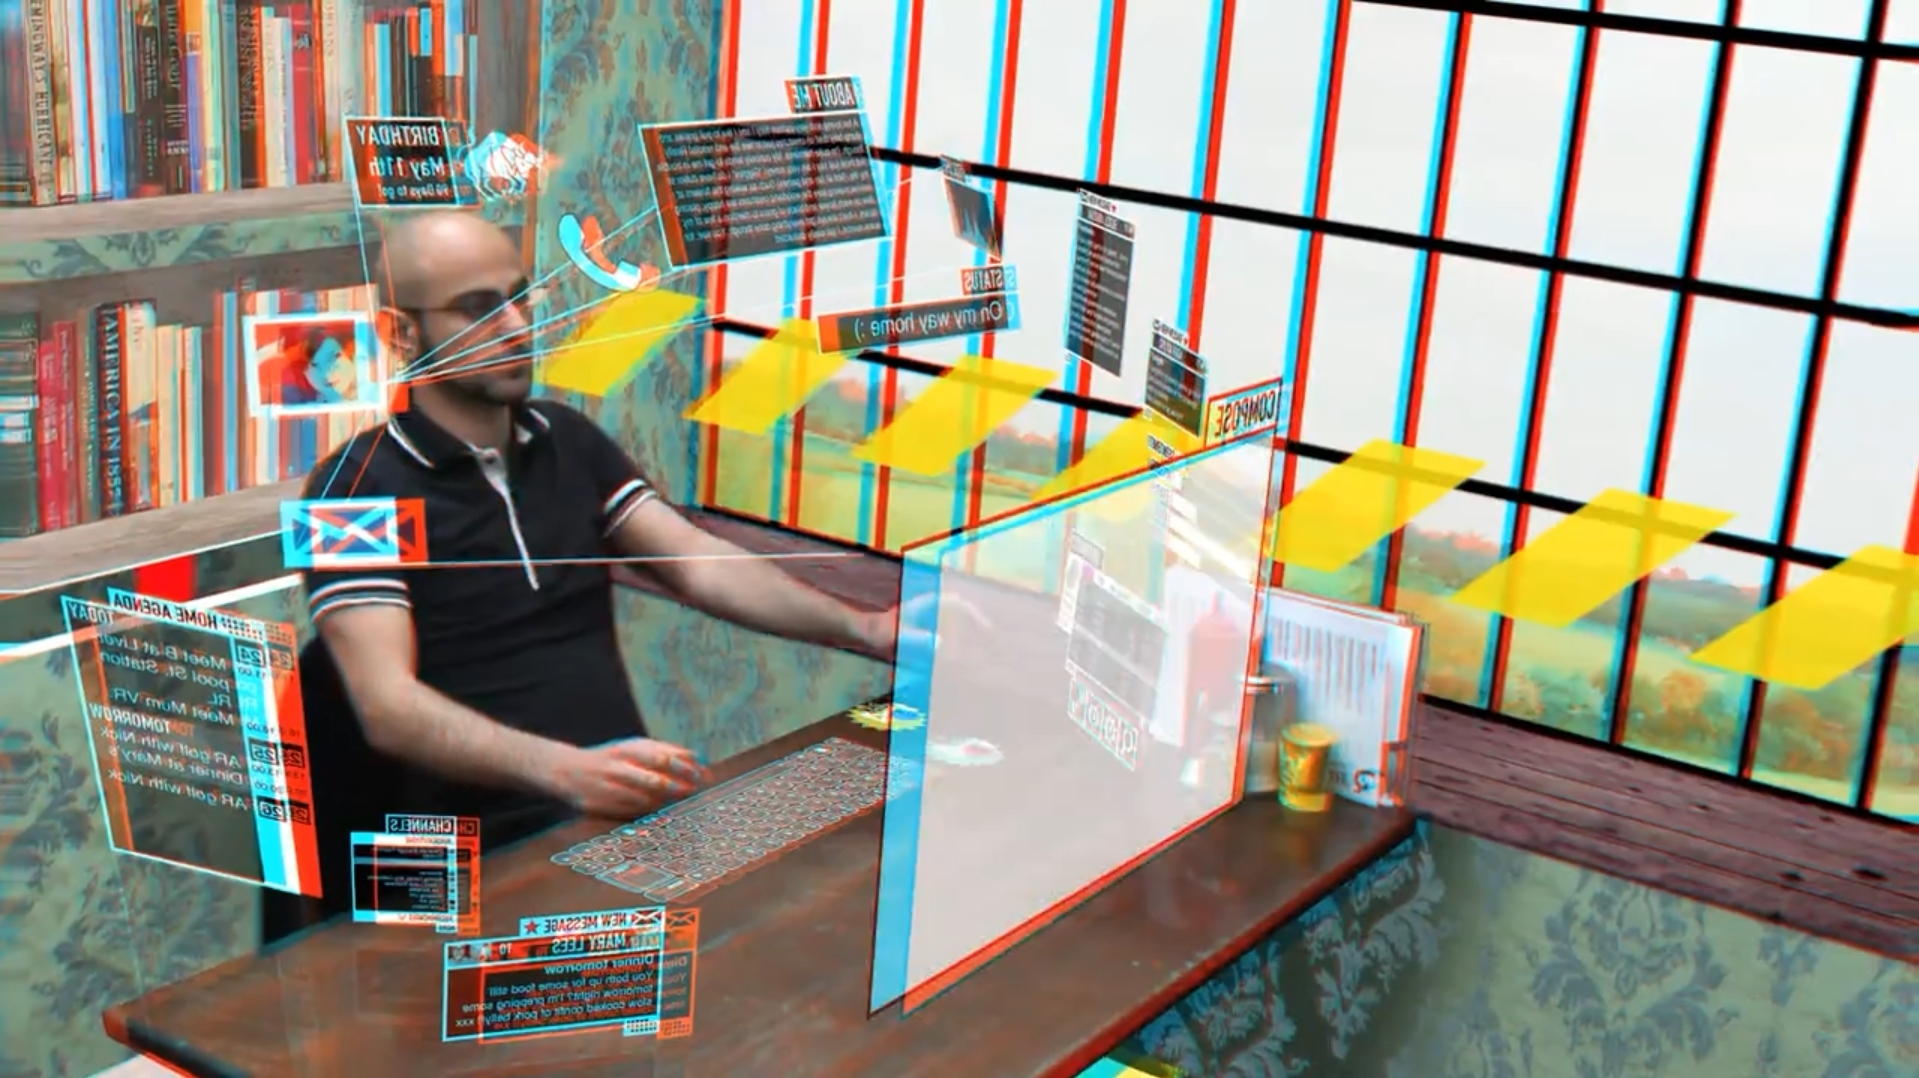
\includegraphics[width=100mm]{images/arcity_01.jpg}}
  \end{center}
  \caption{『Augmented City 3D』における自身環境を展開している描写}
  \label{fig:arcity01}
\end{figure}

また、机に横になった状態であっても画面を見られるよう、ディスプレイが視界内に収まるよう配置された描写もあり(図\ref{fig:arcity02})、実世界のPCディスプレイ以上の機能充実が得られている事についても類似性を見出すことができる。

\begin{figure}[htbp]
  \begin{center}
     \fbox{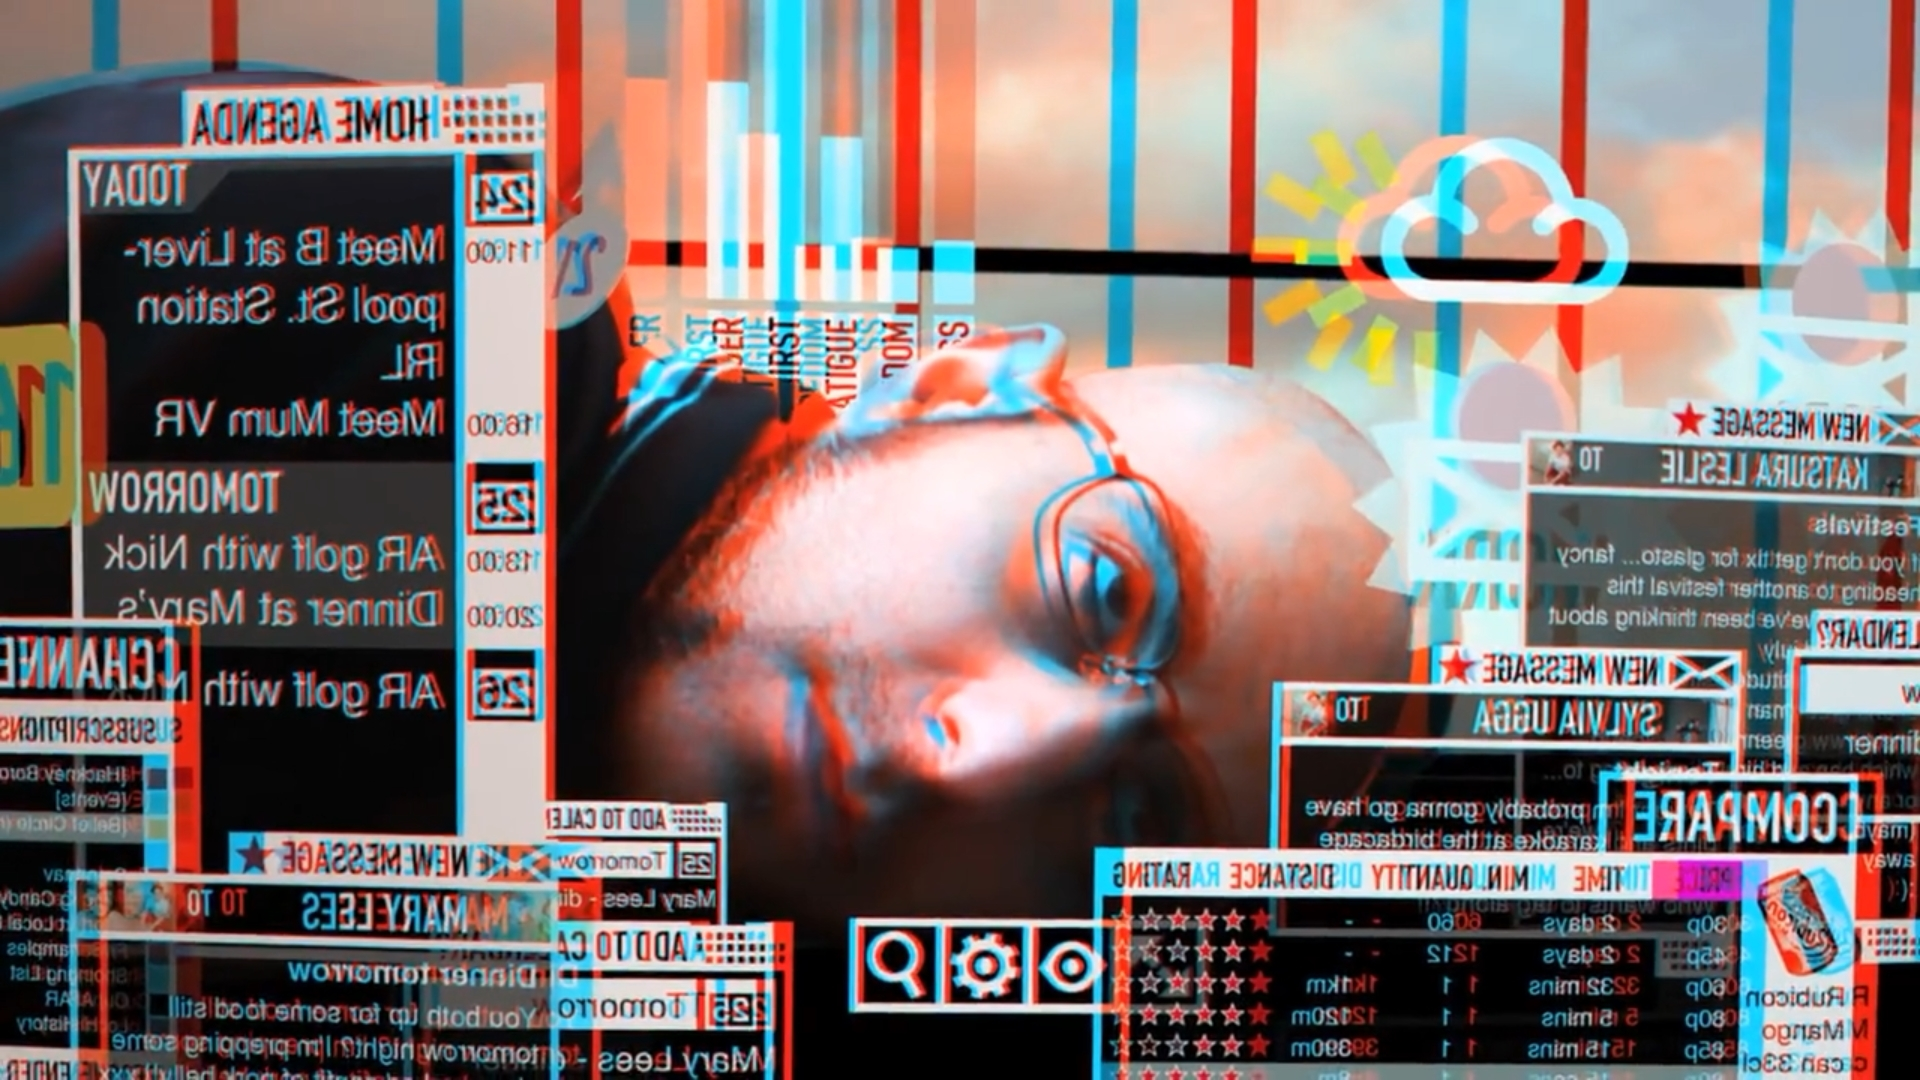
\includegraphics[width=100mm]{images/arcity_02.jpg}}
  \end{center}
  \caption{『Augmented City 3D』におけるディスプレイが視界内に収まるよう配置された図}
  \label{fig:arcity02}
\end{figure}

自身の環境を再現する上でプライベート性は重要な要素となるが、『Augumented city 3D』では、仮想的な壁によって、自身の視点でのプライベート性を再現していた(図\ref{fig:arcity03})。このように、見たくないものを隠すという付加的な機能は、日常的に利用できる場面が多い。例えば、PCや家電の配線を隠すための配線ボックスやクローゼットの扉などは、ARによって代替する事ができる。また、作業に集中する為に、自身を囲うように閉じた空間を仮想的に作り出したり、汚い部屋を掃除するのが面倒なため、その部分を仮想的な壁で隠して、綺麗な側面のみを演出することも可能である。

\begin{figure}[htbp]
  \begin{minipage}{0.5\hsize}
    \begin{center}
      \fbox{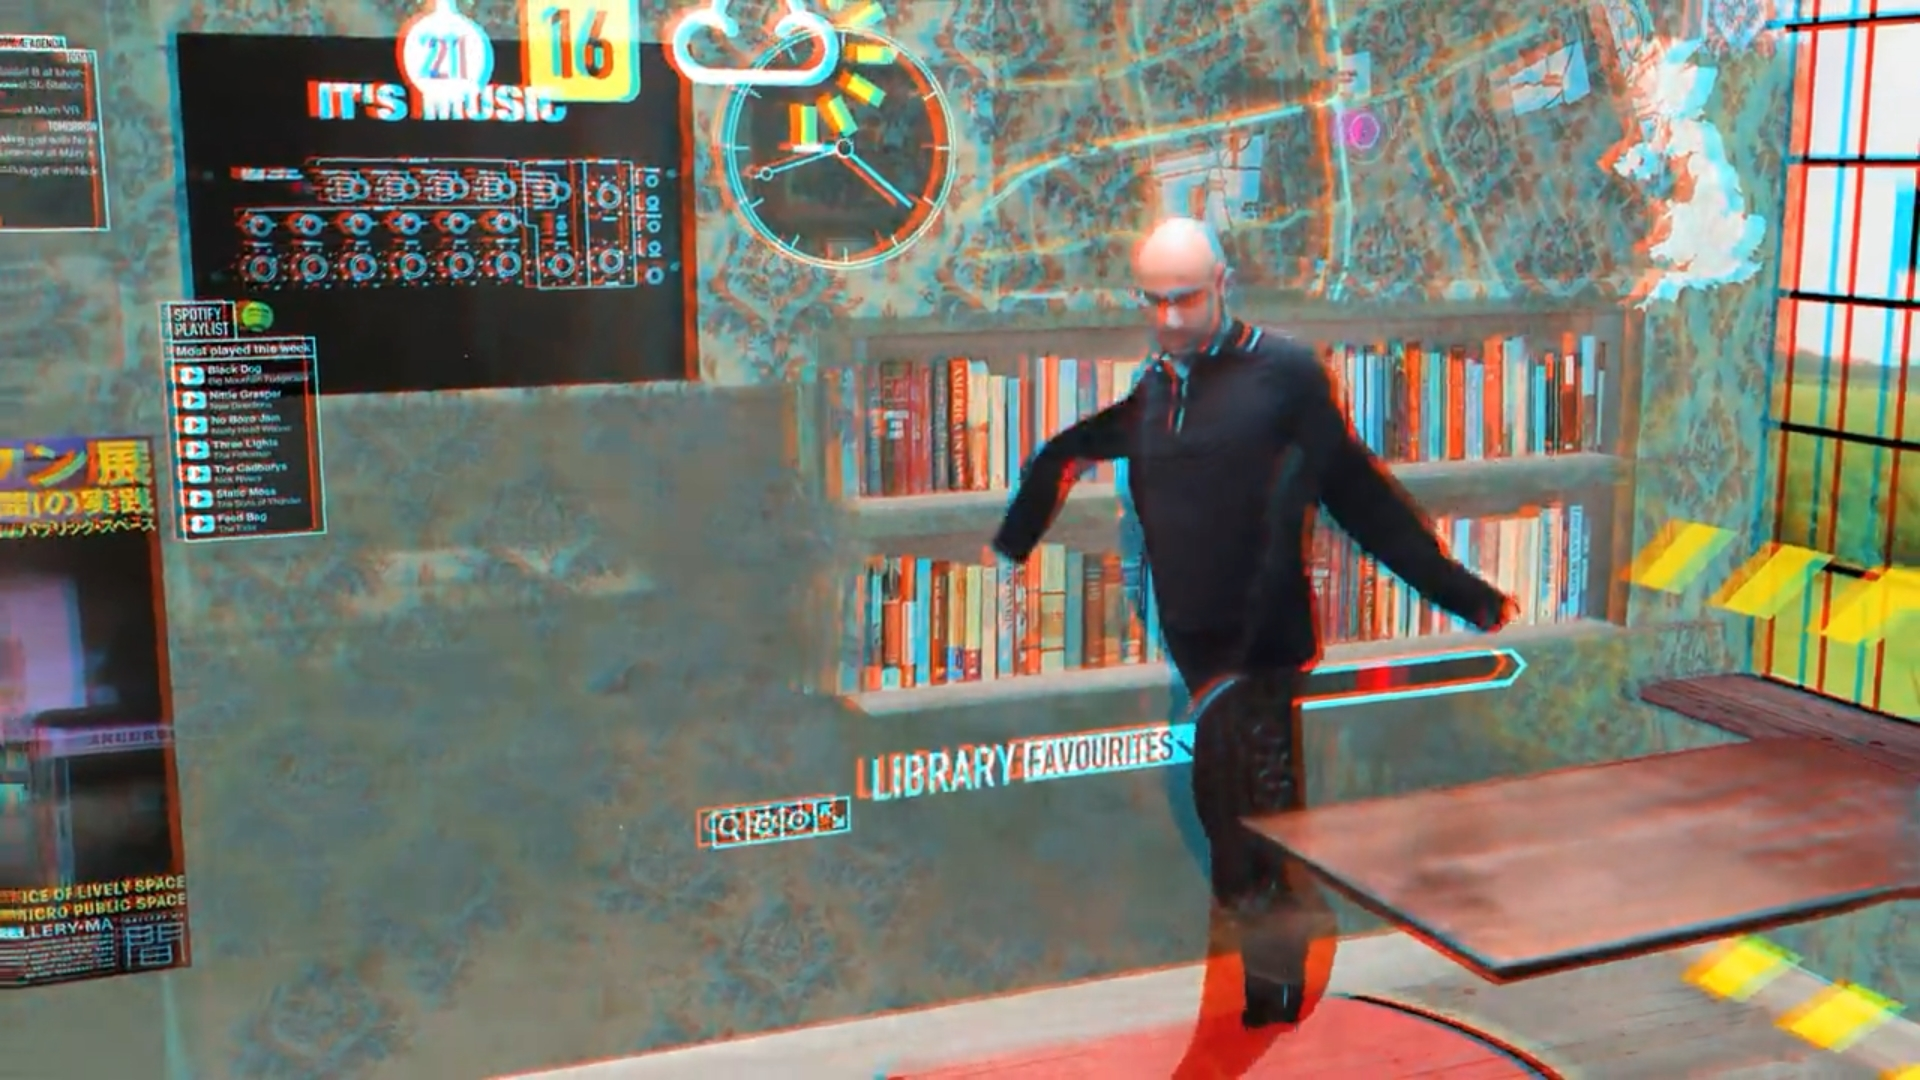
\includegraphics[width=60mm]{images/arcity_03.jpg}}
    \end{center}
  \end{minipage}
  \begin{minipage}{0.5\hsize}
    \begin{center}
      \fbox{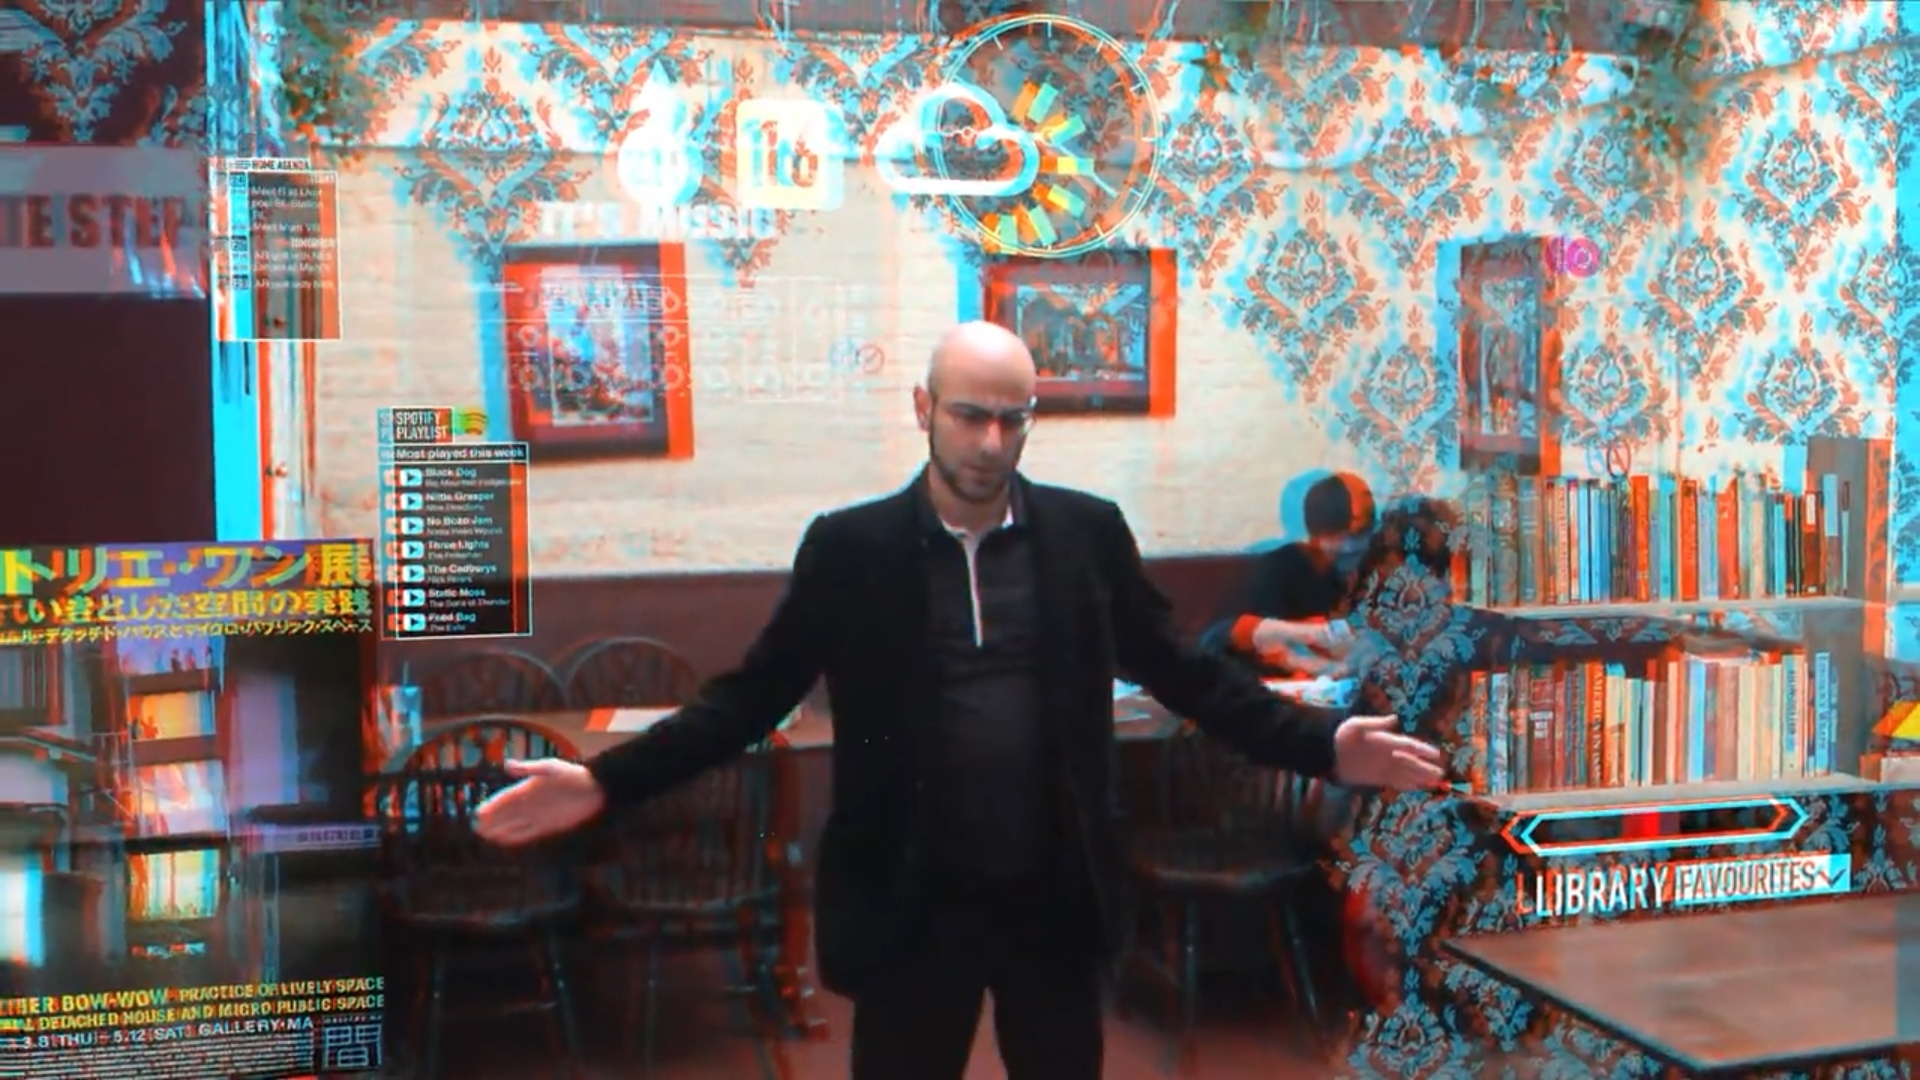
\includegraphics[width=60mm]{images/arcity_04.jpg}}
    \end{center}
  \end{minipage}
  \caption{『Augmented City 3D』におけるプライベート性を再現する描写}
  \label{fig:arcity03}
\end{figure}


\section{アニメ『PSYCHO-PASS』におけるARを用いた見た目の変更}

2012年に放送されたテレビアニメ『PSYCHO-PASS』\cite{psycopass}では、主人公の部屋の見た目を、その日の好みに合わせて変更する描写がある(図\ref{fig:psycho})。見た目の上書きという点では、簡素化支援システムとは異なっている。しかし、一般的にデザインされたインテリアが好まれるように、見た目が整っていることも、生活の機能充実の一つと捉えられる。現在は、見た目と機能を合わせて一つのモノとしているが、それらを切り分け、見た目も簡素化支援システムの対象とすることで、全てが無個性な白い部屋に仮想的なデザインを上乗せする事も可能である。

\begin{figure}[htbp]
  \begin{minipage}{0.5\hsize}
    \begin{center}
      \fbox{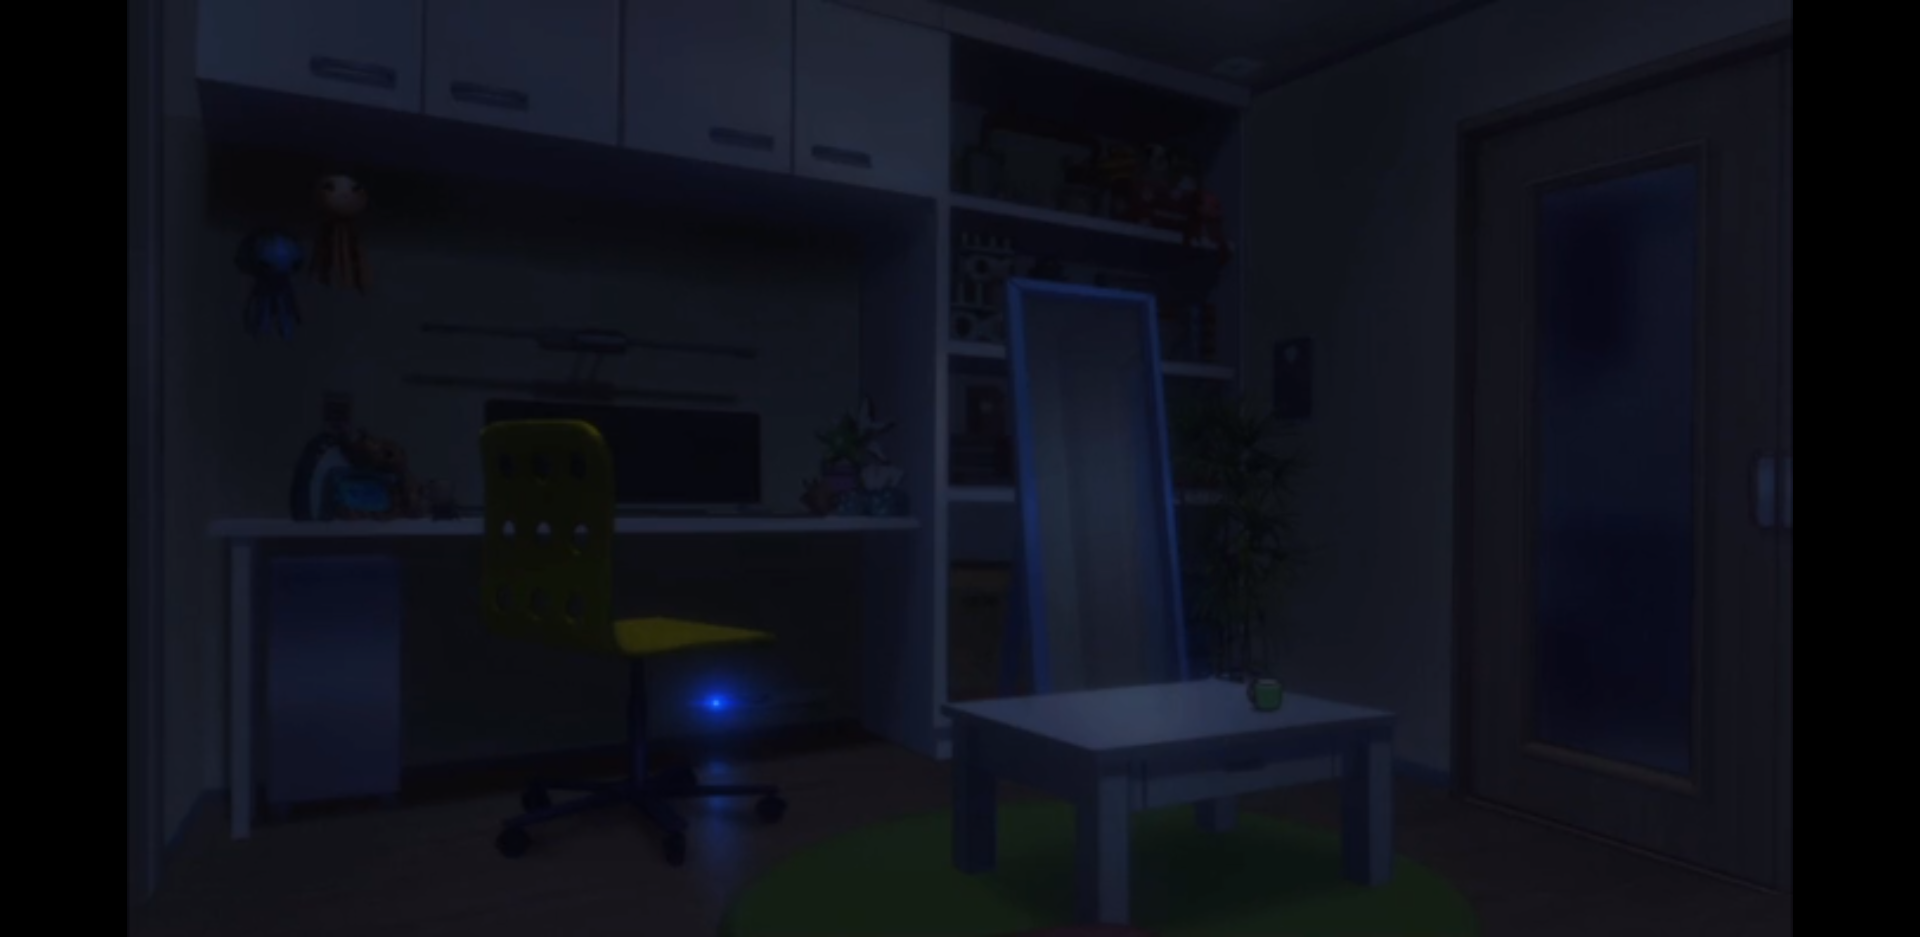
\includegraphics[width=60mm]{images/psycopass_01.png}}
    \end{center}
  \end{minipage}
  \begin{minipage}{0.5\hsize}
    \begin{center}
      \fbox{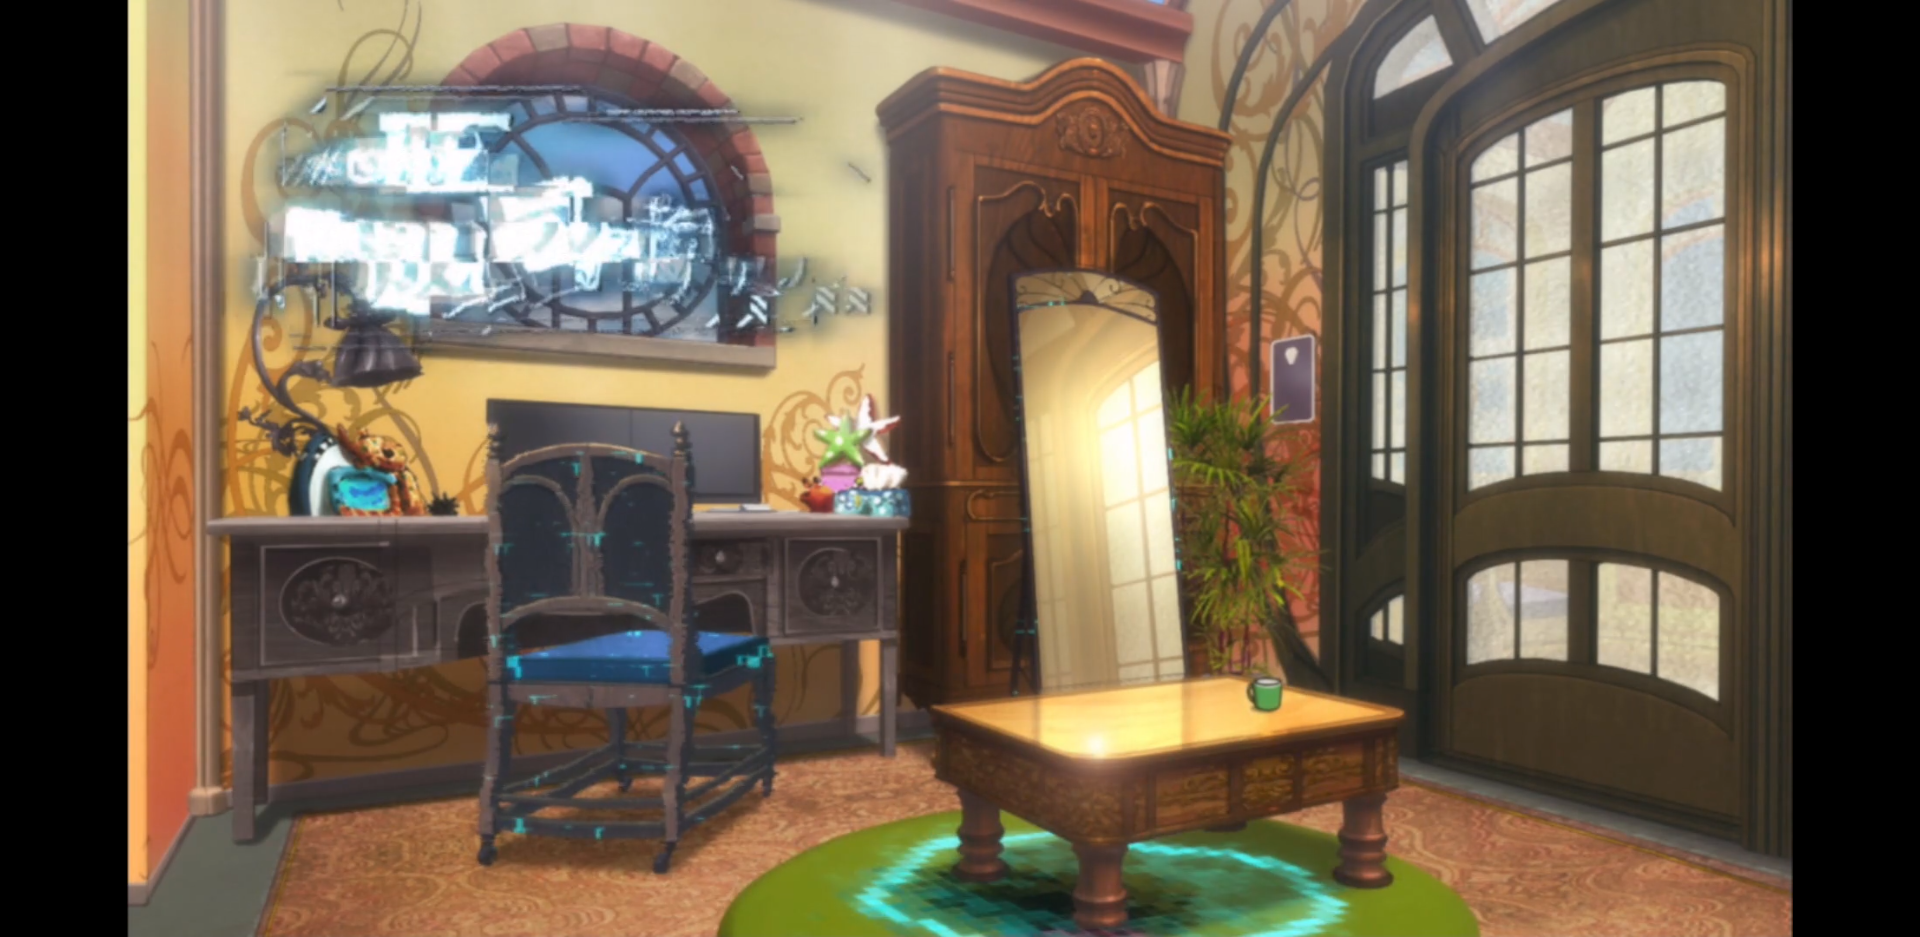
\includegraphics[width=60mm]{images/psycopass_02.png}}
    \end{center}
  \end{minipage}
  \caption{『PSYCHO-PASS』における部屋の見た目の変更の描写の前後}
  \label{fig:psycho}
\end{figure}

\section{没入型ディスプレイ技術『CAVE』}

CAVE(Cave Automatic Virtual Environment)\cite{cave}はプロジェクションマッピングを用いた没入型環境で、プロジェクターで部屋内の正面、左右面、床面に立体映像を投影することで、広視野の映像体験を実現するシステムである。部屋内にいるだけで、容易に没入体験をすることができるという点で、様々な分野に利用されている。主に仮想現実を体験するための装置として用いられるが、現実に重ねて投影している点では、拡張現実技術として考えることも可能である。

簡素化支援システムは日常的に利用される事が前提の為、体験者に負担がないCAVEは、使用するデバイスとして適していると考えられる。


